
\documentclass[11pt,titlepage,a4paper]{report}

%INCLUSIONE PACCHETTI
%---------------------------------------------
\usepackage[italian]{babel}
\usepackage{fancyhdr}
\usepackage{graphicx}
\graphicspath{{./pics/}} % cartella di salvataggio immagini

% STILE DI PAGINA
%---------------------------------------------
\pagestyle{fancy}
\renewcommand{\sectionmark}[1]{\markright{\thesection.\ #1}}
\lhead{\nouppercase{\rightmark}}
\rhead{\nouppercase{\leftmark}}
\renewcommand{\chaptermark}[1]{%
\markboth{\thechapter.\ #1}{}}

%Ridefinisco lo stile plain della pagina
\fancypagestyle{plain}{%
	\lhead{
\includegraphics[height=50pt]{logo.eps}}
	\chead{}
	\rhead{HappyCode inc \\ happycodeinc@gmail.com}
	\lfoot{BR-jsys}
	\cfoot{\thepage}
	\renewcommand{\headrulewidth}{1pt}
	\renewcommand{\footrulewidth}{1pt}
}
% layout
\begin{document}
%definizione variabili 
\newcommand{\lv}{ 2.0 } % latest version
\newcommand{\dt}{ Modifiche ai documenti }% Document title
\newcommand{\Grammatica}{} % paragrafo dove si trova la spiegazione della grammatica
%common variables
\newcommand{\br}{\underline{business rule}}
\newcommand{\brs}{\underline{business rules}}
\newcommand{\bo}{\underline{business object}}
\newcommand{\bos}{\underline{business objects}}
\newcommand{\rp}{\underline{repository}}
\newcommand{\brp}{BusinessRuleParser}
\newcommand{\brl}{BusinessRuleLexer}
\newcommand{\BR}{\underline{BusinessRule}}

%nomi dei componenti
\newcommand{\AT}{Alessia Trivellato}
\newcommand{\ET}{Elena Trivellato}
\newcommand{\FC}{Filippo Carraro}
\newcommand{\LA}{Luca Appon}
\newcommand{\MB}{Michele Bortolato}
\newcommand{\MT}{Marco Tessarotto}
\newcommand{\MM}{Mattia Meroi}%altre variabili
% ultime versioni dei documenti da modificare solo alla fine
\newcommand{\AR}{AnalisiDeiRequisiti.2.6.pdf}
\newcommand{\DdP}{DefinizioneDiProdotto.0.9.pdf}
\newcommand{\G}{ Glossario.1.8.pdf }
\newcommand{\NdP}{NormeDiProgetto.2.0.pdf}
\newcommand{\PdQ}{ PianoDiQualifica.2.0.pdf }
\newcommand{\PdP}{ PianoDiProgetto.1.7.pdf }
\newcommand{\ST}{SpecificaTecnica.1.5.pdf}
\newcommand{\TR}{TestReport.0.7.pdf}
\newcommand{\MU}{ManualeUtente.0.3.pdf}%nomi documenti
%fine definizione variabili
\hyphenation{
 a-na-lo-go
 as-so-cia-zio-ne
 %attività non si può inserire come tutte le parole accentate che vanno messe nel testo semplice scritte at\-ti\-vi\-tà o come variabile
 coe-ren-za
 com-po-nen-ti
 des-crit-te
 des-cri-zio-ni
 di-a-gram-ma
 di-a-gram-mi
 e-le-men-to
 e-se-gui-re
 e-si-sten-ti
 es-pli-ci-to
 glo-bal-men-te
 glos-sa-rio
 li-vel-lo
 ne-ces-sa-rio
 per-met-te-re
 re-po-si-to-ry
 re-vi-sio-na-men-to
 ri-chies-te
 se-gna-la-ta
 va-li-da-zio-ne
 va-ria-bi-li
 ve-ri-fi-ca-re
 vi-sua-liz-za-te
 e-ven-tua-li
 o-pe-ra-zio-ne
 ar-chi-via-zio-ne
 mo-di-fi-ca
}


%sillabazione
\begin{titlepage}
\begin{center}
\vspace*{0.5in}

\includegraphics{logo.eps}
\vspace*{0.2in}

{\Large \textbf{BR-jsys}}
{\Large \emph{business rules} per sistemi gestionali in architettura J2EE } 
\vspace{2in}

\Huge \textsc{ \dt }

\end{center}
\end{titlepage}
\vspace*{0.5in}%pagina del titolo

\begin{center}
\thispagestyle{plain}
\begin{table}[htbp]
\large{
\begin{tabular}{l}
\Large{\textbf{\textsf{Capitolato: ``BR-jsys''}}} \\
\begin{tabular}{|p{6cm}|p{6cm}|} \hline
\textbf{Data creazione:} & 15/03/2008 \\ \hline
\textbf{Versione:} & \lv \\ \hline
\textbf{Stato del documento:} & Formale, esterno \\ \hline
% ----------------------------------------------------------------------------autori
\textbf{Redazione:} &  \MT \\ \hline
\textbf{Revisione:} & \FC \\ \hline
\textbf{Approvazione:} & \MM \\ \hline
\end{tabular} \\
\end{tabular}
}
\end{table}

\begin{table}[hbtp]
\large{
\begin{tabular}{l}
\Large{\textbf{\textsf{Lista di distribuzione}}} \\

\begin{tabular}{|p{6cm}|p{6cm}|} \hline
{HappyCode inc}& Gruppo di lavoro\\ \hline
{Tullio Vardanega, Renato Conte}& Rappresentanti del committente \\ \hline
{Zucchetti S.r.l}& Azienda committente\\ \hline
\end{tabular} \\
\end{tabular}
}
\end{table}
\begin{table}[hbtp]

\Large{\textbf{\textsf{Diario delle modifiche}}} \\
\begin{small}
\begin{tabular}[t]{|p{1,2cm}|p{1.9cm}|p{2.9cm}|p{5cm}|} \hline
Versione & Data & Autore & Descrizione \\ \hline
%-------------------------------------------------------------------------------diario modifiche
0.1 & 15/03/2008 & \MT & Prima stesura del documento \\ \hline
0.2 & 15/03/2008 & \AT & Modifiche apportate ai vari documenti \\ \hline
0.1 & 15/03/2008 & \MT & Prima stesura del documento \\ \hline


\end{tabular} \\
\end{small}

\end{table}
\end{center}
\newpage

\tableofcontents 
\chapter*{Sommario}
\addcontentsline{toc}{chapter}{I Sommario}
Il presente documento contiene la descrizione delle modifiche apportate ai precedenti documenti consegnati alla Revisione di Qualifica sostenuta marted\`i 11 marzo. In generale, per quanto riguarda tutti i documenti, \`e stata sottolineata solo la prima occorrenza dei termini riportati nel ``\G''.
\section*{Come leggere il documento}
Ogni capitolo qui presente rappresenta il nome del documento a cui si riferisce. L'ultimo capitolo presenta invece i miglioramenti che potrebbero essere apportati in futuro al documento ``BR-jsys''.
\chapter{Glossario}
Sono stati aggiunti i seguenti due termini: \\
\begin{itemize}
\item \textbf{Jivelint}: Strumento che esegue l'analisi statica su codice sorgente Java. Esso trover\`a il codice e le variabili inutilizzate, oltre a molti altri errori. \\
\item \textbf{JUnit}: Struttura di supporto alla procedura usata per verificare singole parti di codice sorgente. Viene utilizzato per il linguaggio di programmazione Java. 
\end{itemize}

\chapter{Analisi dei Requisiti}
Essendo deprecato, il requisito F9 non verr\`a soddisfatto in questa sede. La struttura del nostro codice sorgente non preclude per\`o la possibilit\`a di aggiungere questa funzionalit\`a successivamente al nostro prodotto.
\chapter{Norme di Progetto}
La tabella ``Diario delle modifiche'' prensente a pag 2, \`e stata spezzata al fine di migliorare la formattazione.
\chapter{Piano di Qualifica}
Nel ``Piano di qualifica'' \`e stata aggiunta una sezione contenente gli esiti dei test (dei difetti e di convalida), come da richiesta. La sezione inserita \`e visibile nel documento ``TestReportDelta.1.0.pdf'' .


\chapter{Piano di Progetto}
Il documento ``\PdP'' precedentemente consegnato, \`e stato sostituito dal documento ``PianoConsuntivo.0.1.pdf''.
Per quanto riguarda gli errori segnalati a questo documento, la mancanza dei dati a consuntivo in ingresso alla Revisione di Qualifica sono da attribuirsi solo a un mancato aggiornamento della data delle tabelle relative alla fase di sviluppo. 
\chapter{Specifica Tecnica}
Sono state apportate correzioni:
\begin{itemize}
\item ai vizi di forma presenti nel paragrafo 1.1;
\item \`e stata tolta la sottolineatura alla parola ``tokenStream'';
\item sono state aggiunte le sottolineature ai nomi degli oggetti contenuti nei diagrammi delle attivit\`a.
\end{itemize}
\begin{center} 
\section{Inserimento business rule nel repository}
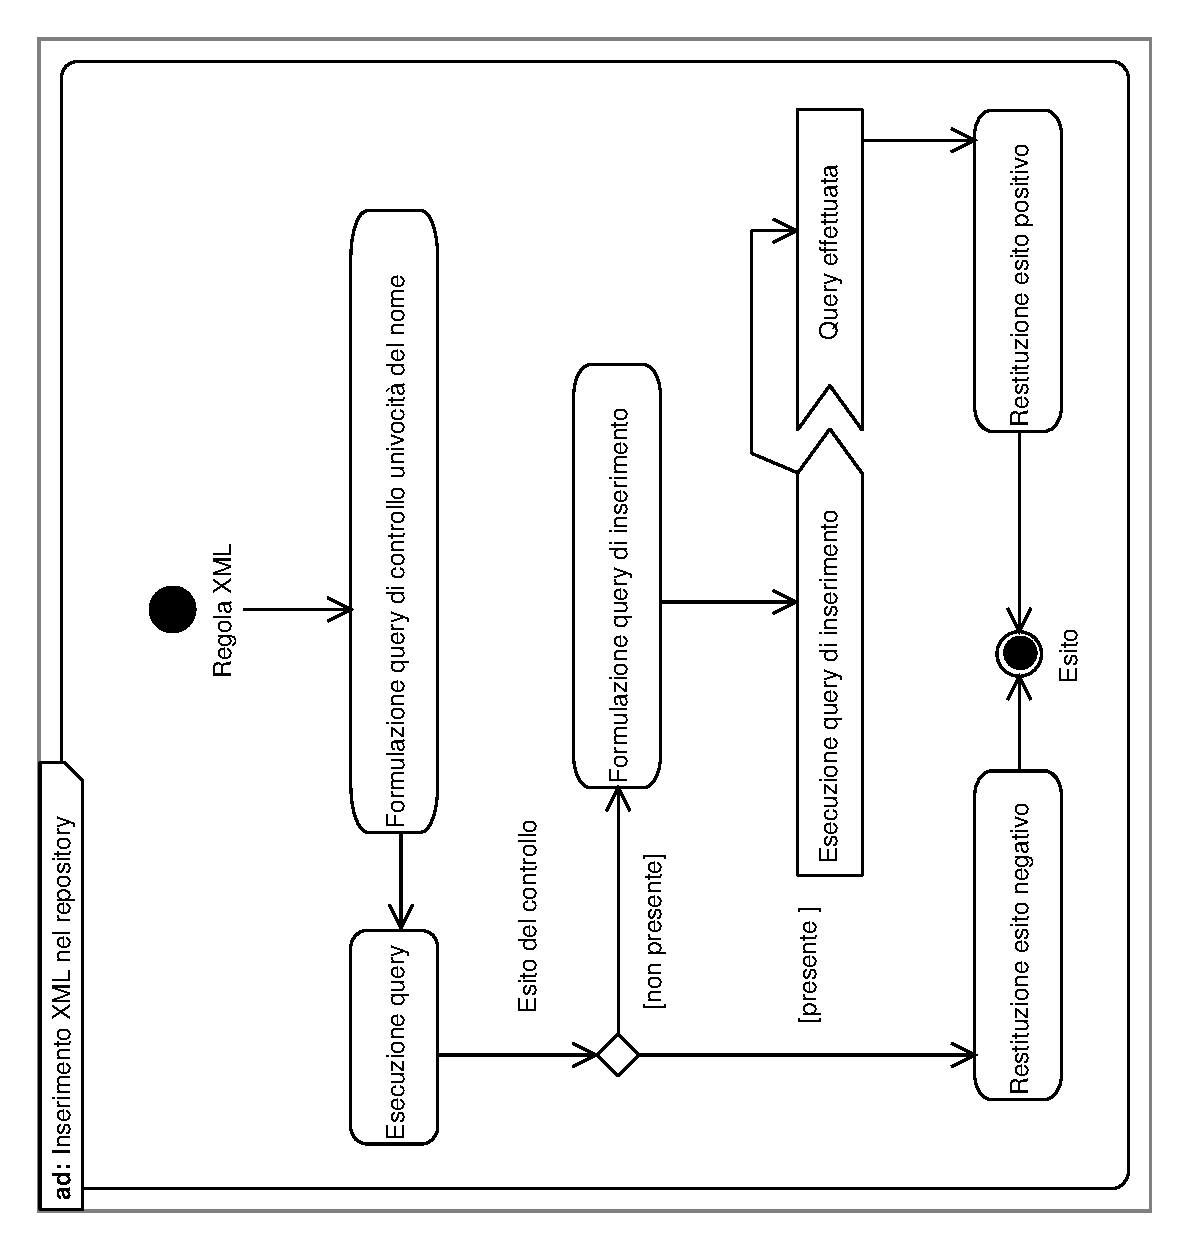
\includegraphics[width=0.9\textwidth, angle=-90]{activity-dia/InserimentoXMLnelrepository.eps}
\end{center}
Si dovr\`a prima di tutto controllare che il nome della regola si vuole inserire non sia gi\`a presente nel \rp. Se \`e gi\`a presente si troncher\`a immediatamente l'operazione di inserimento, altrimenti sar\`a formulata la query adatta per inserire la \br . La query verr\`a inviata al DBMS eXist dal quale si attender\`a poi l'esito dell'inserimento (si \`e scelto di utilizzare i blocchi di ``invio segnale'' e ``ricezione segnale'' per evidenziare una situazione di attesa). Si indicher\`a solo successivamente al chiamante che l'operazione \`e riuscita con successo.
\chapter{Manuale Utente}
Il documento ``\MU'' \`e gi\`a stato allegato in versione definitiva.
\chapter{Test Report}
Il documento ``TestReportDelta.1.0.pdf'' integra il ``\TR'' precedentemente consegnato e approvato.
\chapter{Miglioramenti desderabili}
In questo capitolo elencheremo i miglioramenti che potrebbero essere apportati al prodotto ``BR-jsys'', ma che non siamo riusciti a implementare per motivi di tempo e costi. 
\begin{itemize}
\item \textbf{Normalizzazione di business rules:} rendere possibile la normalizzazione delle business rule, ovvero ogni qualvolta si riscontra un tab, uno spazio, un \textbackslash t, un \textbackslash r, \textbackslash n si devono trasformare in un singolo spazio. 
\item \textbf{Operazioni tra stringhe:} rendere possibili altre operazioni, oltre al confronto, sulle stringhe. Ad esempio la concatenazione e le operazioni di confronto tra stringhe (\textless, \textgreater); 
\item \textbf{Parentesi tra AND/OR:} rendere possibile la parentesizzazione tra AND e/o OR. Allo stato attuale \`e possibile inserire le parentesi nel nostro linguaggio solo:
\begin{itemize}
\item nelle funzioni matematiche, ad es. SUM(..), COUNT(..), AVG(..);
\item tra espressioni matematiche, ad es (a+b)*c.
\end{itemize}
\item \textbf{Aggiunta di espressioni FLOWR:} rendere possibile la formulazione di query complesse, in stile FLOWR.
\end{itemize}
\end{document}
